\chapter{Basic Concepts}
\label{chapter:intro}

Before proceeding forward it is necessary to understand some of the basic concepts behind hijacking the control flow of an executable and how they evolved into Return Oriented Programming.

\section{Terminology}
\label{sec:payload}

Throughout this paper I will refer to the creation of the ROP \textbf{payload} and injection through an \textbf{exploit / vulnerability}. To better understand the concept let's consider the following analogy: at a customs office someone is trying to smuggle in contraband through a secret passage. The payload represents the contraband we are trying to introduce and the exploit represents the method of delivery, in this case the secret passage. If there is no contraband the secret passage is useless by itself, similarly the contraband is of no use if without a method to smuggle it in.

Other common terms used in the security world are \textbf{attack vector} and \textbf{attack surface}. The former represents the path or means an attacker uses to reach his target, in this context the attack vector is represented by the Return Oriented Programming technique. The latter represents the sum of all attack vectors present which can be used by the attacker.

\section{Stack Smashing Attack}
\label{sec:stacksmash}

One of the traditional exploits\cite{aleph1996stacksmash} used by attackers was to try and manipulate the call stack by taking advantage of a bug in the program, usually a buffer overflow. This happens when a function does not perform proper bounds checking and accepts more input data than it can store properly. The excess data can overflow on the stack and overwrite the return address (\labelindexref{Figure}{fig:stackoverflow}), which can be used to hijack the control flow. The first step of the attack consists of creating a malicious payload with the intent to run arbitrary code, followed by overwriting the return address of a function call to point to the previously injected code.

The buffer overflow exploit has been a favorite technique for attackers over the years and proved to be quite versatile\cite{taeho1999adv.overflow}.

\begin{figure}[htp]%[!tbp]
	\centering
	\subfloat[Initial Buffer]{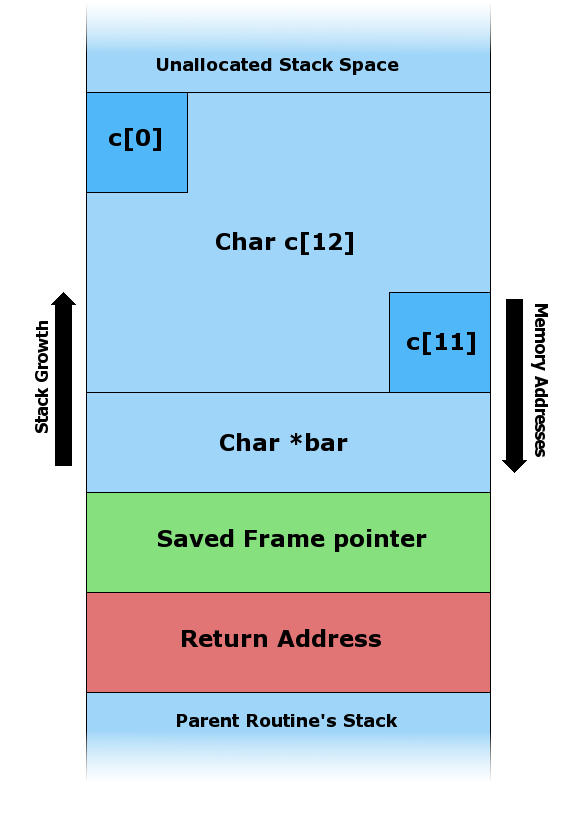
\includegraphics[width=0.3\textwidth]{src/img/stackoverflow1.png}\label{fig:f1}}
	% \hfill
	\subfloat[No Buffer Overflow]{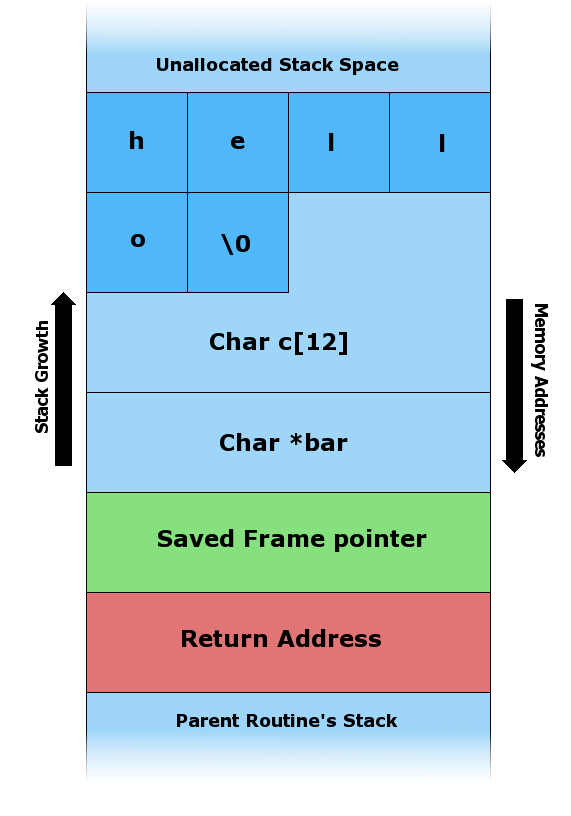
\includegraphics[width=0.3\textwidth]{src/img/stackoverflow2.png}\label{fig:f2}}
	% \hfill
	\subfloat[Buffer Overflow]{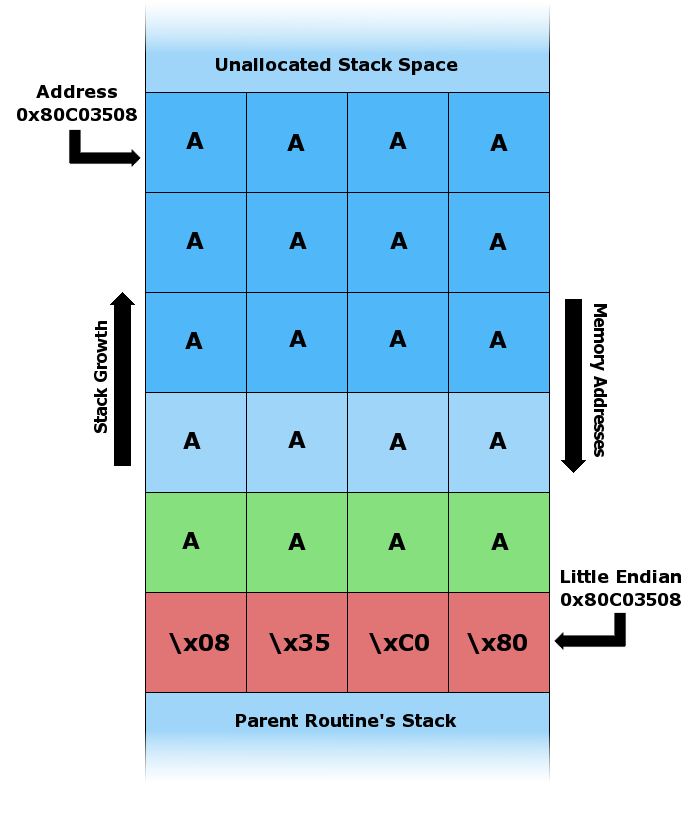
\includegraphics[width=0.35\textwidth]{src/img/stackoverflow3.png}\label{fig:f3}}
	\caption[Stack Smashing Example]{%
		Stack Smashing Example%
		% \footnote{\url{https://en.wikipedia.org/wiki/Stack_buffer_overflow}}%
		\footnotemark
		% \footnote{Random footnote}%
	}
	\label{fig:stackoverflow}
\end{figure}

\footnotetext{\url{https://en.wikipedia.org/wiki/Stack_buffer_overflow}}


\section{Data Execution Prevention}
\label{sec:dep}

In order to prevent attackers from exploiting buffer overflows with this simple technique, modern architectures now implement a Data Execution Prevention\cite{peslyak1997dep} (often referred to as DEP or W\textasciicircum X) mechanism which marks the writable regions of memory as non-executable. This guarantees that no region in the memory can be both executable and writable at the same time. Even if an attacker manages to inject a payload and overwrite the return address with the payload location, when the code will jump and try to execute the malicious code it will cause an exception and the program will crash.

\section{Return to libc}
\label{sec:ret2libc}

Because of the DEP mechanism the attacker is now restricted to code already marked as executable from the memory. Since shared libraries, such as libc, contain subroutines for system calls and other potentially useful functions for an attack, instead of writing a payload onto the stack, the target will now be to overwrite the return address with the entry location of a library function.

Even with this technique\cite{peslyak1997ret2libc}\cite{nergal2001ret2libc} it is difficult to mount a successful attack since most libraries began to remove or restrict functions that would potentially be useful for an attack as a security measure.

\section{Return Oriented Programming}
\label{sec:rop}

Return Oriented Programming can be see as an enhanced ret2libc attack, with the generalization that instead of using whole functions it only uses short assembly instruction sequences already in memory, called gadgets. Each gadget normally executes a very specific and simple task, such as moving a register or incrementing a value for example. In order to chain these gadgets together and create a payload it is ideal to find those gadgets which end in a return instruction (i.e. ret on x86), this will make the instruction pointer jump to the next address on the stack, thus chaining the gadgets together. \labelindexref{Figure}{img:ropattack} illustrates how the stack looks during a ROP attack, each gadget on the stack representing an address for jumping to a specific place in memory to execute the small portion of code (the actual gadget) before jumping back onto the stack to the next gadget address.

\fig[scale=0.4]{src/img/rop-attack-fig-transparent.png}{img:ropattack}{Stack During ROP Attack}

Using gadgets proves more resilient to security measures because no matter what functions or calls are removed or restricted from a library, or any large body of executable code, it will inevitably contain useful gadgets which can be used to mount an attack. By using gadgets as the building blocks for this technique it also gains several advantages over the traditional ret2libc:
\begin{itemize}
	\item Provided enough gadgets, it is Turing-complete
	\item Not limited to function calls
\end{itemize}

The applicability and power of the technique has been proven on different architectures\cite{roemer2012rop} along with the definition of efficient algorithms for analyzing and discovering ROP gadgets.

Currently this technique requires building hand-crafted ROP chains, which can be a tedious and error-prone process. Furthermore the user must have a deep understanding of low level programming as well as the specific architecture on which the executable runs.

